\section{Charakterisierung des Datensatzes}
\label{sec:Charakterisierung}
Der genutzte Datensatz stammt von der Website \href{https://www.kaggle.com/}{kaggle}.
Diese ist eine Website auf der Datensätze geteilt werden können.
Dies ermöglicht es den Nutzern*innen diese zu analysieren oder zum Beispiel damit ein Neuronales Netzwerk zu trainieren.
\\\\
Der genutzte Datensatz trägt den Namen \href{https://www.kaggle.com/ikarus777/best-artworks-of-all-time}{Best Artworks of All Time}.
Es wurde dieser Datensatz gewählt, da in dem Datensatz viele bekannte Gemälde enthalten sind.
Zudem deckt der Datensatz eine große Spanne an bekannten Genre und Künstlern ab.
So gibt er eine gute Stichprobe an Bildern von bekannten Genre.
%Die Bilder des Datensatzes wurden von dem Ersteller des Datensatzes von der Website \href{http://artchallenge.ru/?lang=en}{artchallenge.ru} kopiert.
Der Datensatz besteht dabei aus drei Datein.
\\
Einer "artists.csv"-Datei in der die Namen, und die Genre der Kunstwerke der Künstler*innen gespeichert sind.
In der "artists.csv"-Datei sind zudem einige weitere Daten wie zum Beispiel die Nationalität der Künstler*innen zu finden.
Diese Daten werden allerdings nicht für das Neuronale Netzwerk genutzt, da explizit nur aus den Bildern selber das Genre des Bildes ermittlet werden soll.
Die im Datensatz enthaltenen Künstler*innen sind in Tabelle \ref{tab:artist} im Anhang \ref{sec:anhang} zu finden.
Zudem sind in der Tabelle die Genre, die den Gemälde der Künstler*innen zugeordnet werden und die Anzahl der Bilder des Künstlers*in im Datensatz zu finden.
In Summe beinhaltet der Datensatz 8446 Bilder von 50 verschiedenen Künstlern*innen.
\\
Des weiteren besteht der Datensatz aus einem "images.zip"-Ordner in dem alle Bilder in voller Auflösung gespeichert sind.
Dabei befinden sich im "images.zip"-Ordner 50 weitere Ordner.
Die Ordner tragen jeweils den Namen von einem der Künstler*innen und beinhalten alle Bilder des jeweilgen Künstlers*in die in dem Datensatz vorhanden sind.
\\
Der letzte Teil des Datensatz ist der "resized.zip"-Ordner.
In diesem befinden sich ebenfalls alle Bilder allerdings ohne die Ordner Struktur von "images.zip" und die Größe der Bilder wurde bereits geändert.
Aus diesem Grund ist der "resized.zip"-Ordner ebenfalls irrelevant für den weiteren Verlauf.
\\\\
Einige Beispiel Bilder sind in Abbildung \ref{fig:bilder_datensatz} zu sehen.
In diesem Fall ist deutlich zu erkennen, dass die Bilder unterschiedlichen Genre angehören, diese Unterscheidung ist allerdings nicht immer so einfach.
Ein Beispiel für Bilder bei denen es schwer ist das Genre zu bestimmen wird im Verlauf des Abschnitts \ref{sec:ergebnisse} gezeigt.
\begin{figure}
    \centering
    \caption{Drei Beispiel Bilder aus drei verschiedenen Genre von bekannten Künstlern.}
    \begin{subfigure}{0.30\textwidth}
        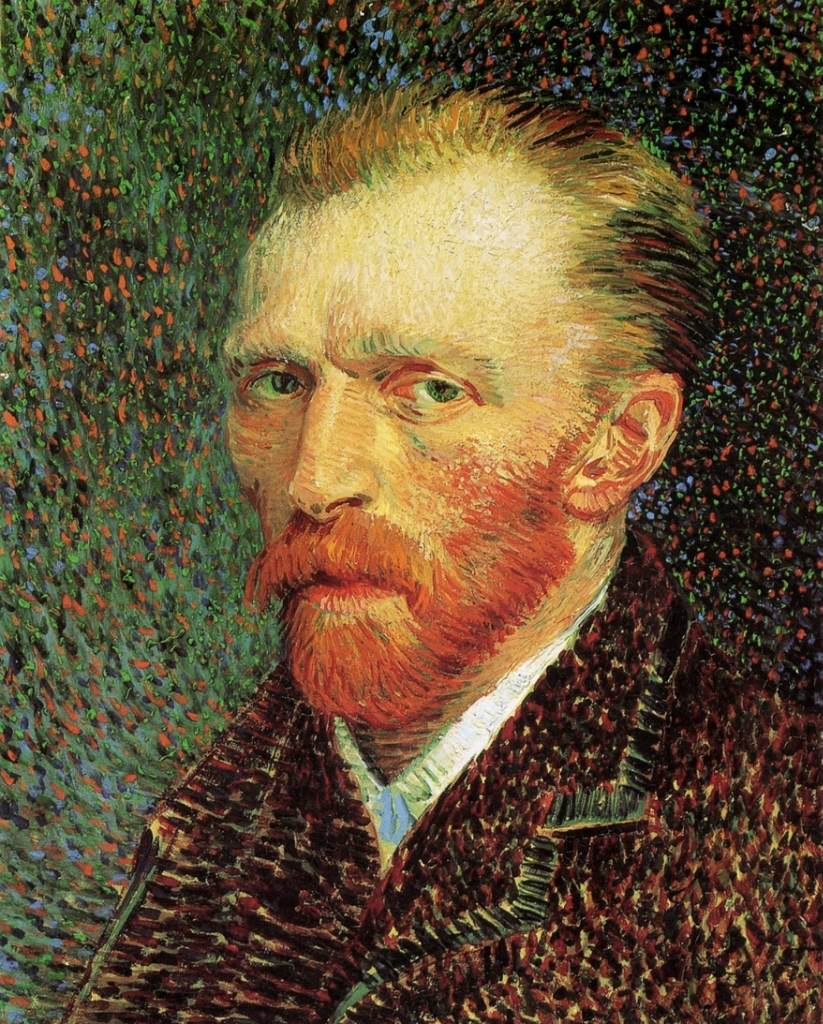
\includegraphics[width=\linewidth]{content/data/Vincent_van_Gogh_582.jpg}
        \caption{"Selbstbildnis", Vincent van Gogh 1887, Öl auf Karton, Post-Impressionismus}
        \label{fig:6}
    \end{subfigure}\hfil % <-- added
    \begin{subfigure}{0.30\textwidth}
      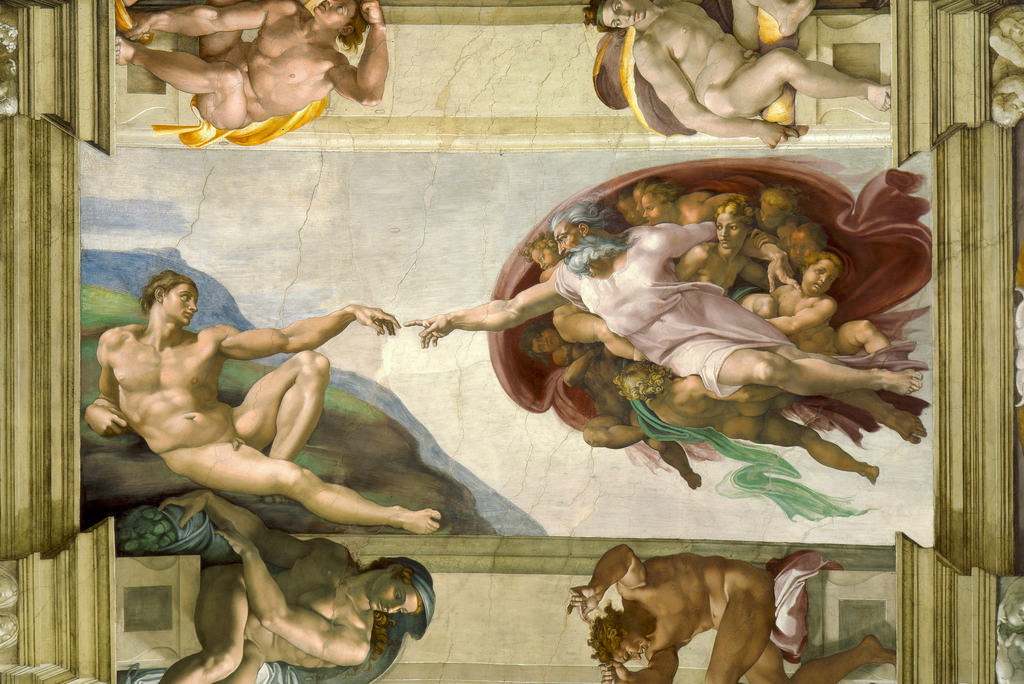
\includegraphics[width=\linewidth]{content/data/Michelangelo_4.jpg}
      \caption{"Die Erschaffung Adams", Michelangelo zwischen 1508 und 1512, ein Fresko in der Sixtinischen Kapelle, Hochrenaissance}
      \label{fig:2}
    \end{subfigure}\hfil % <-- added
    \begin{subfigure}{0.30\textwidth}
      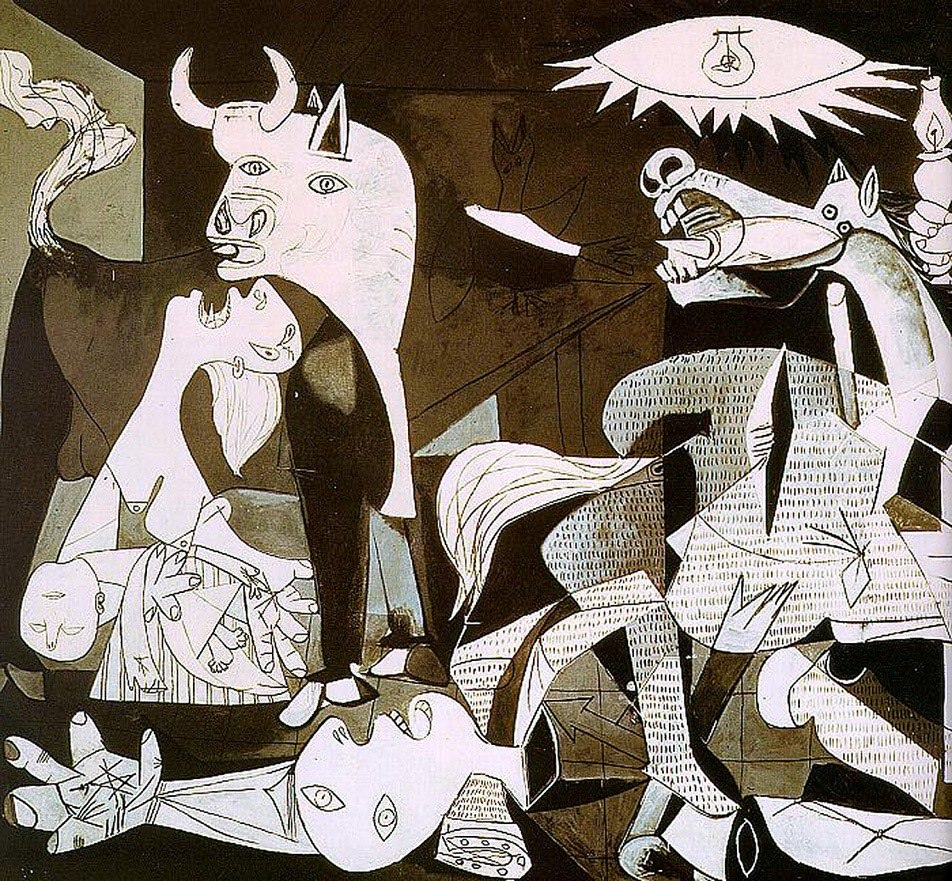
\includegraphics[width=\linewidth]{content/data/Pablo_Picasso_270.jpg}
      \caption{"Guernica", Pablo Picasso 1937, Öl auf Leinwand, Ausschnitt des Orginals, Kubismus}
      \label{fig:4}
    \end{subfigure}\hfil % <-- added
    \label{fig:bilder_datensatz}
\end{figure}